\begin{minipage}{0.45\linewidth}
  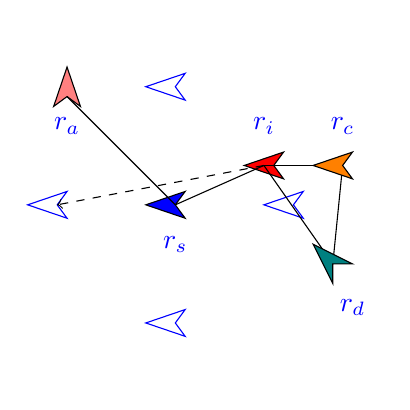
\begin{tikzpicture}
    \useasboundingbox (1,0.5) rectangle (5.5,5);
    % center 2.875 2.75
    \coordinate (S) at (2.875, 2.75);
    \def\shifty{1}
    \def\ddy{2.5}
    \coordinate (A) at (1.5, 4.125);
    \coordinate (B) at (4,4.25-\shifty);
    \draw[fill=blue] (3,2.92) -- (2.5,2.75) -- (3,2.58) -- (2.875,2.75) -- cycle;
    \def\offset{0.5}
    \node[color=blue] at (2.875, 2.75-\offset) {$r_s$};
    % vacancies
    \def\dx{1.5}
    \def\dy{1.5}
    \draw[color=blue] (3+\dx,2.92) -- (2.5+\dx,2.75) -- (3+\dx,2.58) -- (2.875+\dx,2.75) -- cycle;
    \draw[color=blue] (3-\dx,2.92) -- (2.5-\dx,2.75) -- (3-\dx,2.58) -- (2.875-\dx,2.75) -- cycle;
    \draw[color=blue] (3,2.92+\dy) -- (2.5,2.75+\dy) -- (3,2.58+\dy) -- (2.875,2.75+\dy) -- cycle;
    \draw[color=blue] (3,2.92-\dy) -- (2.5,2.75-\dy) -- (3,2.58-\dy) -- (2.875,2.75-\dy) -- cycle;
    % another two robots
    \draw[fill=red!50] (1.5,4.5) -- (1.33,4) -- (1.5,4.125) -- (1.67,4) -- cycle; % center .5 4.125
    \node[color=blue] at (1.5, 3.25+\offset) {$r_a$};
    \def\shiftx{1.25}
    \draw[fill=red] (3+\shiftx,3.42) -- (2.5+\shiftx,3.25) -- (3+\shiftx,3.08) -- (2.875+\shiftx,3.25) -- cycle;          
    \node[color=blue] at (4, 4.75-\shifty) {$r_i$};
    \draw[] (S) -- (A);
    \draw[] (S) -- (B);
    \coordinate (V) at (2.875-\dx,2.75);
    \draw[dashed, ->] (B) -- (V);
    % two children of r_i
    \coordinate (C) at  (5, 3.25);
    %\draw[fill=orange] (5,3.5) -- (4.83,3) -- (5, 3.25) -- (5.17,3) -- cycle; % center .\5 3.625
    \node[color=blue] at (5, 3.75) {$r_c$};
    % center or r_c
    \def\xcc{5}
    \def\ycc{3.25}
    \def\hrlen{0.375}
    \def\ylen{0.17}
    \def\xlen{0.125}
    \coordinate (CC) at (\xcc, \ycc);
    % center of r_d
    \def\xdc{4.875}
    \def\ydc{2}
    \def\longlen{0.25}
    \coordinate (DC) at (\xdc, \ydc);
    \draw[] (B) -- (CC);
    \draw[] (B) -- (DC);
    \draw[] (CC) -- (DC);
    \coordinate (CA) at (\xcc-\hrlen, \ycc);
    \coordinate (CB) at (\xcc+\xlen, \ycc+\ylen);
    \coordinate (CD) at (\xcc+\xlen, \ycc-\ylen);
    \draw[fill=orange] (CA) -- (CB) -- (CC) -- (CD) -- cycle;
    \coordinate (D) at (5.375-\offset, 4.5-\ddy);

    \node[color=blue] at (5.125, 3.95-\ddy) {$r_d$};

  
    \coordinate (DA) at (\xdc-\longlen, \ydc+\longlen);
    \coordinate (DB) at (\xdc, \ydc-\longlen);
    \coordinate (DD) at (\xdc+\longlen, \ydc);
    \draw[fill=teal] (DA) -- (DB) -- (DC) -- (DD) -- cycle;
  \end{tikzpicture}
\end{minipage}
\begin{minipage}{0.45\linewidth}
  \centering
  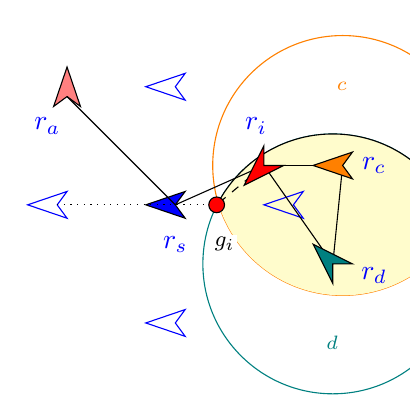
\begin{tikzpicture}
    \tikzstyle{ann} = [fill=white, font=\footnotesize,inner sep=1pt]   
    \useasboundingbox (1,0.5) rectangle (5.5,5);
    % center 2.875 2.75
    \def\xs{2.875}
    \def\ys{2.75}
    \coordinate (S) at (\xs, \ys);
    \def\shiftx{1.25}               
    \def\shifty{1}
    \def\ddy{2.5}
    \def\offset{0.5}
    \def\movedist{1.65}
    \coordinate (A) at (1.5, 4.125);
    \coordinate (B) at (4,4.25-\shifty); % r_i
    \def\xrc{5}
    \def\yrc{3.25}
    \coordinate (C) at (\xrc, \yrc);
    \def\xrd{4.875}
    \def\yrd{2}
    \coordinate (D) at (\xrd, \yrd);
     % ranges of r_c and r_d
    \def\childcircleD{(D) circle (\movedist)}
    \def\childcircleC{(C) circle (\movedist)}
    \draw[orange] \childcircleC;
    \draw[teal] \childcircleD;
    % intersection region of children's ranges
    \begin{scope}
      \clip \childcircleC;
      \filldraw[fill=yellow!20] \childcircleD;
    \end{scope}
    
    \draw[fill=blue] (3,2.92) -- (2.5,2.75) -- (3,2.58) -- (2.875,2.75) -- cycle;
    \node[color=blue] at (2.875, 2.75-\offset) {$r_s$};
    \draw[fill=red!50] (1.5,4.5) -- (1.33,4) -- (1.5,4.125) -- (1.67,4) -- cycle; % center .5 4.125
    % vacancies
    \def\dx{1.5}
    \def\dy{1.5}
    \draw[color=blue] (3+\dx,2.92) -- (2.5+\dx,2.75) -- (3+\dx,2.58) -- (2.875+\dx,2.75) -- cycle;
    \draw[color=blue] (3-\dx,2.92) -- (2.5-\dx,2.75) -- (3-\dx,2.58) -- (2.875-\dx,2.75) -- cycle;
    \draw[color=blue] (3,2.92+\dy) -- (2.5,2.75+\dy) -- (3,2.58+\dy) -- (2.875,2.75+\dy) -- cycle;
    \draw[color=blue] (3,2.92-\dy) -- (2.5,2.75-\dy) -- (3,2.58-\dy) -- (2.875,2.75-\dy) -- cycle;
   
    \node[color=blue] at (1.25, 3.25+\offset) {$r_a$};
    %%%%%%%%%%%%%%%% triangle facing -135 degree
    \def\xc{4}
    \def\yc{3.25}
    \coordinate (TC) at (\xc, \yc);
    \def\longlen{0.25}
    \coordinate (TA) at (\xc-\longlen, \yc-\longlen);
    \coordinate (TB) at (\xc, \yc+\longlen);
    \coordinate (TD) at (\xc+\longlen, \yc);
 
    %%%%%%%%%%%%%%%%%%%%%%%%%%%%%%%%%%%%%%%%%%%%%
    \node[color=blue] at (3.9, 4.75-\shifty) {$r_i$};
    \draw[] (S) -- (A);
    \draw[] (S) -- (B);
  
    \node[color=blue] at (5.4, 3.25) {$r_c$};
    \draw[] (B) -- (C);
   
    \node[color=blue] at (5.4, 4.35-\ddy) {$r_d$};
    \draw[] (B) -- (D);
    \draw[] (C) -- (D);
    \coordinate (G) at (1.9+\dx,2.75);
    \draw[dotted] (2.875-\dx,2.75) -- (G);
    \draw[dashed] (B) -- (G);
    \def\goalcircleG{(G) circle (0.1)}
    \draw[fill=red] \goalcircleG;
    \node[ann] at (3.5,2.25) {$g_i$};
    % three robots
    \draw[fill=red] (TA) -- (TB) -- (TC) -- (TD) -- cycle;
    % draw r_c
    \def\xcc{5}
    \def\ycc{3.25}
    \def\hrlen{0.375}
    \def\ylen{0.17}
    \def\xlen{0.125}
    \coordinate (CC) at (\xcc, \ycc);
    \coordinate (CA) at (\xcc-\hrlen, \ycc);
    \coordinate (CB) at (\xcc+\xlen, \ycc+\ylen);
    \coordinate (CD) at (\xcc+\xlen, \ycc-\ylen);
    \draw[fill=orange] (CA) -- (CB) -- (CC) -- (CD) -- cycle;
    %\def\parentCircle {(S) circle (\movedist)}
    %\draw[color=blue] \parentCircle;
    % draw r_d  heading 135 degrees
    \def\xdc{4.875}
    \def\ydc{2}
    \coordinate (DC) at (\xdc, \ydc);
    \coordinate (DA) at (\xdc-\longlen, \ydc+\longlen);
    \coordinate (DB) at (\xdc, \ydc-\longlen);
    \coordinate (DD) at (\xdc+\longlen, \ydc);
    \draw[fill=teal] (DA) -- (DB) -- (DC) -- (DD) -- cycle;
    %%%%%%%%%%%%%% add texts of bounded ranges
    %\node[color=blue] at (\xs-0.75, \ys-\shifty) {$\B_s$};
    \node[color=orange] at (\xrc, \yrc+\shifty) {$\B_c$};    
    \node[color=teal] at (\xrd, \yrd-\shifty) {$\B_d$};
  \end{tikzpicture}
\end{minipage}
 \caption{(a) Robot $r_s$ be a stable robot, it has two neighbors
    $r_a, r_i$ and four vacancies.  Robot $r_i$ is the relocate robot
    and its ultimate destination is the vacancy (hollow) ahead of
    $r_s$.  (b) The relocate robot $r_i$ has two descendants $r_c,
    r_d$ in the moving subtree. Two circles denote the bounded
    ranges of $r_c, r_d$, $r_i$ finds an intermediate goal (red dot)
    $g_i\in\left(\B_c \cap \B_d\right)$.}